Work has been conducted to propose a correction to the SI-method based on the findings in this paper. The idea is to find correction factors that can be applied to the roll damping components calculated with the SI-method. In order to handle the problem of $\hat{B_e}$ accuracy being very much depending on the roll amplitude a roll amplitude correction factor has also added. The correction factors have been determined by fitting a linear regression model to the roll damping components, calculated with the SI-method at roll amplitudes between 0 and 10 degrees, giving the following expression: 
\begin{equation} \label{eq:polynom_correction}
\hat{B_{e}} = 0.7396 \hat{B_{BK}} - 1.256 \hat{B_{E}} + 9.289 \hat{B_{F}} + 0.6891 \hat{B_{L}} + 0.6691 \hat{B_{W}} + 0.02178 phi_{a} - 0.003594
\end{equation}

The proposed correction factors reduce $\hat{B_{BK}}$ and $\hat{B_{W}}$, removes $\hat{B_{E}}$ and $\hat{B_{L}}$ is not corrected much. 

\subsection{Cross validation}
When constructing a regression model from a data set, over-fitting the data can be a problem. Including too many parameters and/or allowing too high order of the model would give a very good representation of the present roll damping data, but large extrapolation errors when the model is used on other data. K-fold cross validation has been used to "mimic" this situation. The data has been split into five smaller sets (folds). Four of the folds are used to train the model and the fifth is used for testing (validation). The validation is done by calculating the coefficient of determination $R^2$ for the fitted model. This is done for all five possible train/test combinations. Applying the proposed correction improves the accuracy according to the cross validation results in table \ref{tab:crossvalidation} with an average $R^2$ of 0.68 compared to 0.47 without the correction. The improvement can also be seen when comparing figure \ref{fig:ikeda_components} with \ref{fig:ikeda_phi_a}.
\begin{tabular}{lrr}
\toprule
{} &  \$R\textasciicircum 2(SI-method)\$ &  \$R\textasciicircum 2(SI-corrected)\$ \\
\midrule
0 &              0.39 &                 0.66 \\
1 &              0.56 &                 0.71 \\
2 &              0.47 &                 0.66 \\
3 &              0.32 &                 0.69 \\
4 &              0.59 &                 0.66 \\
\bottomrule
\end{tabular}


\begin{figure}[H]
\vspace{-0.5cm}
\centering
  \centering
  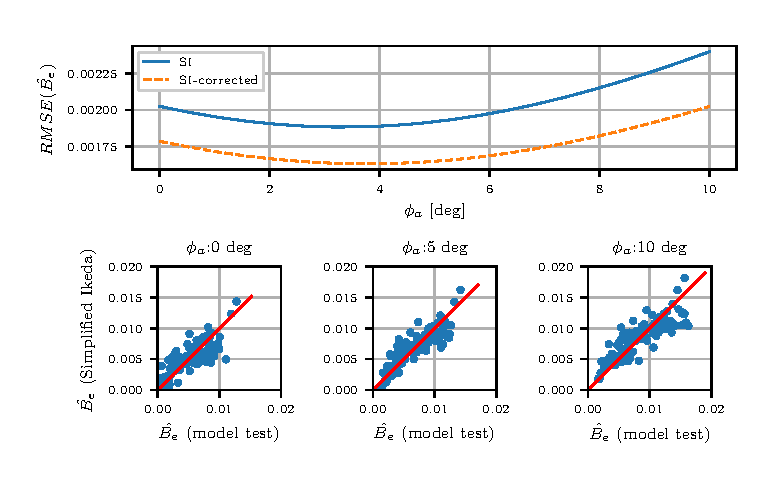
\includegraphics[]{figures/ikeda_corrected_phi_a.eps}
  \vspace{-0.5cm}
  \caption{Root mean square error of roll damping prediction between the SI-method, corrected SI-method and the model test results (upper plot). Influence of roll amplitude $\phi_a$ on $\hat{B_e}$ between the corrected SI-method and model tests for $0^{\circ}$ (bottom left plot), $5^{\circ}$ (bottom middle plot) and $10^{\circ}$ (bottom right plot), respectively.}
  \label{fig:ikeda_phi_a_correction}
\end{figure}
